\documentclass[a4paper,11pt]{ltjsarticle}
\usepackage{graphicx}
\usepackage{luatexja-fontspec}
\usepackage{caption}
\usepackage{amsmath,amssymb,bm,braket}
\usepackage[english]{babel}
\usepackage{multicol}
\usepackage{titlesec}
%\usepackage{gnuplot-lua-tikz}
\usepackage[top=20truemm,bottom=20truemm,left=20truemm,right=20truemm]{geometry}
\usepackage{array}
\usepackage{upgreek}
\usepackage{fancyhdr}
\renewcommand{\refname}{}
\usepackage{listings,jvlisting}
\usepackage{tikz}
\usepackage[thmmarks,amsmath]{ntheorem}
\usepackage[version=3]{mhchem}
\usetikzlibrary{external}
\tikzexternalize
\lstset{
  basicstyle={\ttfamily},
  identifierstyle={\small},
  commentstyle={\smallitshape},
  keywordstyle={\small\bfseries},
  ndkeywordstyle={\small},
  stringstyle={\small\ttfamily},
  frame={tb},
  breaklines=true,
  columns=[l]{fullflexible},
  numbers=left,
  xrightmargin=0pt,
  xleftmargin=3pt,
  numberstyle={\scriptsize},
  stepnumber=1,
  numbersep=1pt,
  lineskip=-0.5ex
}
\captionsetup[figure]{format=plain, labelformat=simple, labelsep=quad,labelfont=bf,name={Fig.}}
\captionsetup[table]{format=plain, labelformat=simple, labelsep=quad,labelfont=bf}
\parindent = 0pt
%[BoldFont=HGSMinchoE]{MSMincho}[BoldFont=HiraMinProN-W6]{HiraMinPro-W3}
\titleformat{\section}{\normalfont\fontsize{9}{10}\bfseries\fontspec{Times New Roman}}{\thesection.}{1em}{}
\usepackage[backend=biber,sorting=none,style=numeric,maxnames=99,minnames=1]{biblatex}
\addbibresource{utility/REFERENCES.bib}
\defbibheading{bibliography}[\refname]{%
  \section*{REFERENCES}%
  \vspace{-7pt}  % ここで空白を調整。お好みの値に変更してください。
}
\newfontfamily\subsectionfont{Times New Roman} % サブセクション用フォント
\titleformat{\subsection}
  {\normalfont\large\bfseries} % サブセクションのフォントを指定
  {\thesubsection}{1em}{}
\renewbibmacro{in:}{}
\renewbibmacro*{journal+issuetitle}{%
  \addcomma\space% カンマとスペースを追加
  \usebibmacro{journal}%
  \setunit*{\addspace}%
  \usebibmacro{volume+number+eid}%
  \setunit{\addspace}%
  \printfield{note}%
  \newunit
}
\renewbibmacro*{volume+number+eid}{
  \printfield{volume}%
  \setunit*{\addnbspace}%
  \printfield{number}%
  \setunit{\addcomma\space}%
  \printfield{eid}
}
\DeclareFieldFormat[article]{volume}{\textbf{#1}}
\DeclareFieldFormat[article]{pages}{#1}
\DeclareFieldFormat{journaltitle}{#1}
\usepackage{hyperref}
\renewenvironment{abstract}{\par\noindent}{\par}
%\pagenumbering{gobble}
\usepackage{docmute}
\usepackage{setspace}
\usepackage{titlesec} % 見出しのカスタマイズ用

% セクションのフォーマットをカスタマイズ
\titleformat{\section}
  {} % フォントサイズとスタイル
  {\Large\bfseries\thesection\ \ }               % 番号の前の内容(空白)
  {0em}            % 番号とタイトルの間の間隔
  {\Large\bfseries}


\theoremstyle{plain}
\theoremheaderfont{\normalfont\bfseries}
\theorembodyfont{\itshape}   % 本文を斜体に
\theoremseparator{.}         % タイトルと本文の区切りを「.」に設定
\newtheorem{definition}{Definition}
\begin{document}
\section{Results}\label{results}{
    \ \ \ Firstly, we perform numerical simulations of the pseudo-3D Surface Code, introduced in Section~\ref{pseudo_pseudo-three-dimensional_surface_code}, using a circuit that executes a 2D Heisenberg model and compare it to the 2D Surface Code. The results are presented in Fig.~\ref{results_of_pseudo_3D}, and a more complex system is shown in Fig.~\ref{results_of_pseudo_3D_1}. In these figures, the horizontal and vertical axes represent the instruction number and distance, respectively, where distance refers to the number of patches required for routing operations.\\

    \begin{figure}[h]
        \centering
        \includegraphics[scale=0.5]{figure/results_pseudo_3D.eps}
        \vspace{-20pt}\caption{}
        \label{results_of_pseudo_3D}
    \end{figure}

    \ \ \ In Fig.~\ref{results_of_pseudo_3D}, the graph illustrates that in the 2D Surface Code, a substantial number of operations exceeded a distance of 30. In contrast, in the 3D Surface Code, the longest operation distance remained below 30. Furthermore, the average distance per operation was significantly reduced from 8.18 in the 2D configuration to 5.36 in the 3D configuration, resulting in an approximately 66\% improvement in overall circuit distance. However, the total time required to execute the entire circuit did not change despite expanding the routing dimension to 3D.

    \begin{figure}[h]
        \centering
        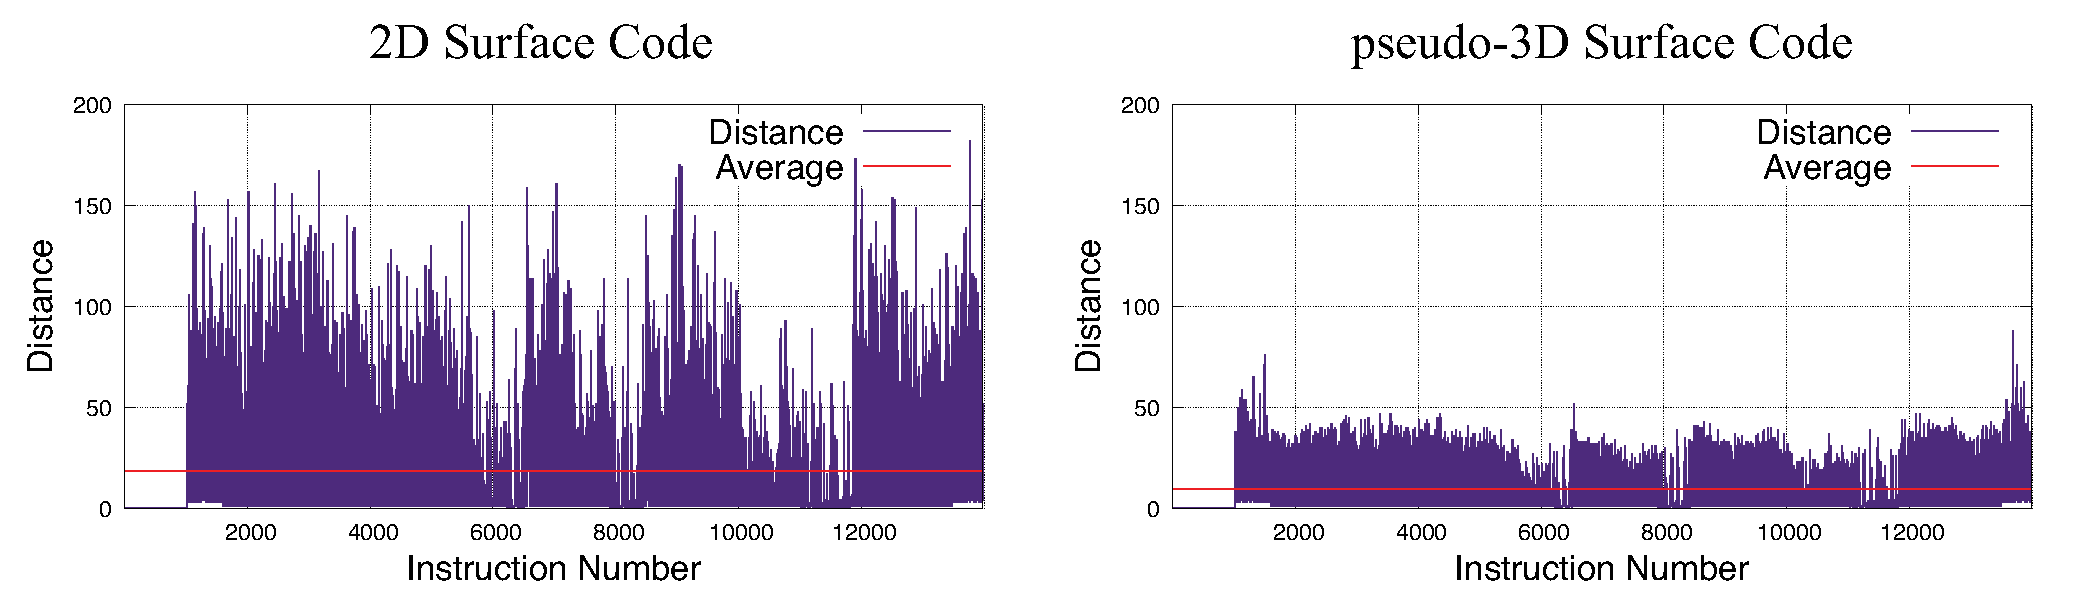
\includegraphics[scale=0.5]{figure/results_pseudo_3D_1.eps}
        \vspace{-20pt}\caption{}
        \label{results_of_pseudo_3D_1}
    \end{figure}

    In the more complex system shown in Fig.~\ref{results_of_pseudo_3D_1}, similar improvements are observed, further demonstrating the effectiveness of the pseudo-3D Surface Code in reducing operation distances. The average distance per operation was significantly reduced from 18.64 in the 2D configuration to 9.74 in the 3D configuration, resulting in an approximately 52\% improvement in overall circuit distance. However, the total time required to execute the entire circuit did not change in the more complex system. Therefore, the pseudo-3D Surface Code does not improve the parallelization of the circuit.
    \clearpage

    \ \ \ Secondly, we perform numerical simulations of the placement optimization method introduced in Section~\ref{placement_optimization}. The results are presented in Fig.~\ref{placement_optimization_2D} for the 2D case and Fig.~\ref{placement_optimization_3D} for the 3D case. Additionally, the graphs which are optimized by the potential energy model are shown in Fig.\ref{} and Fig.\ref{}.
    \begin{figure}[h]
        \centering
        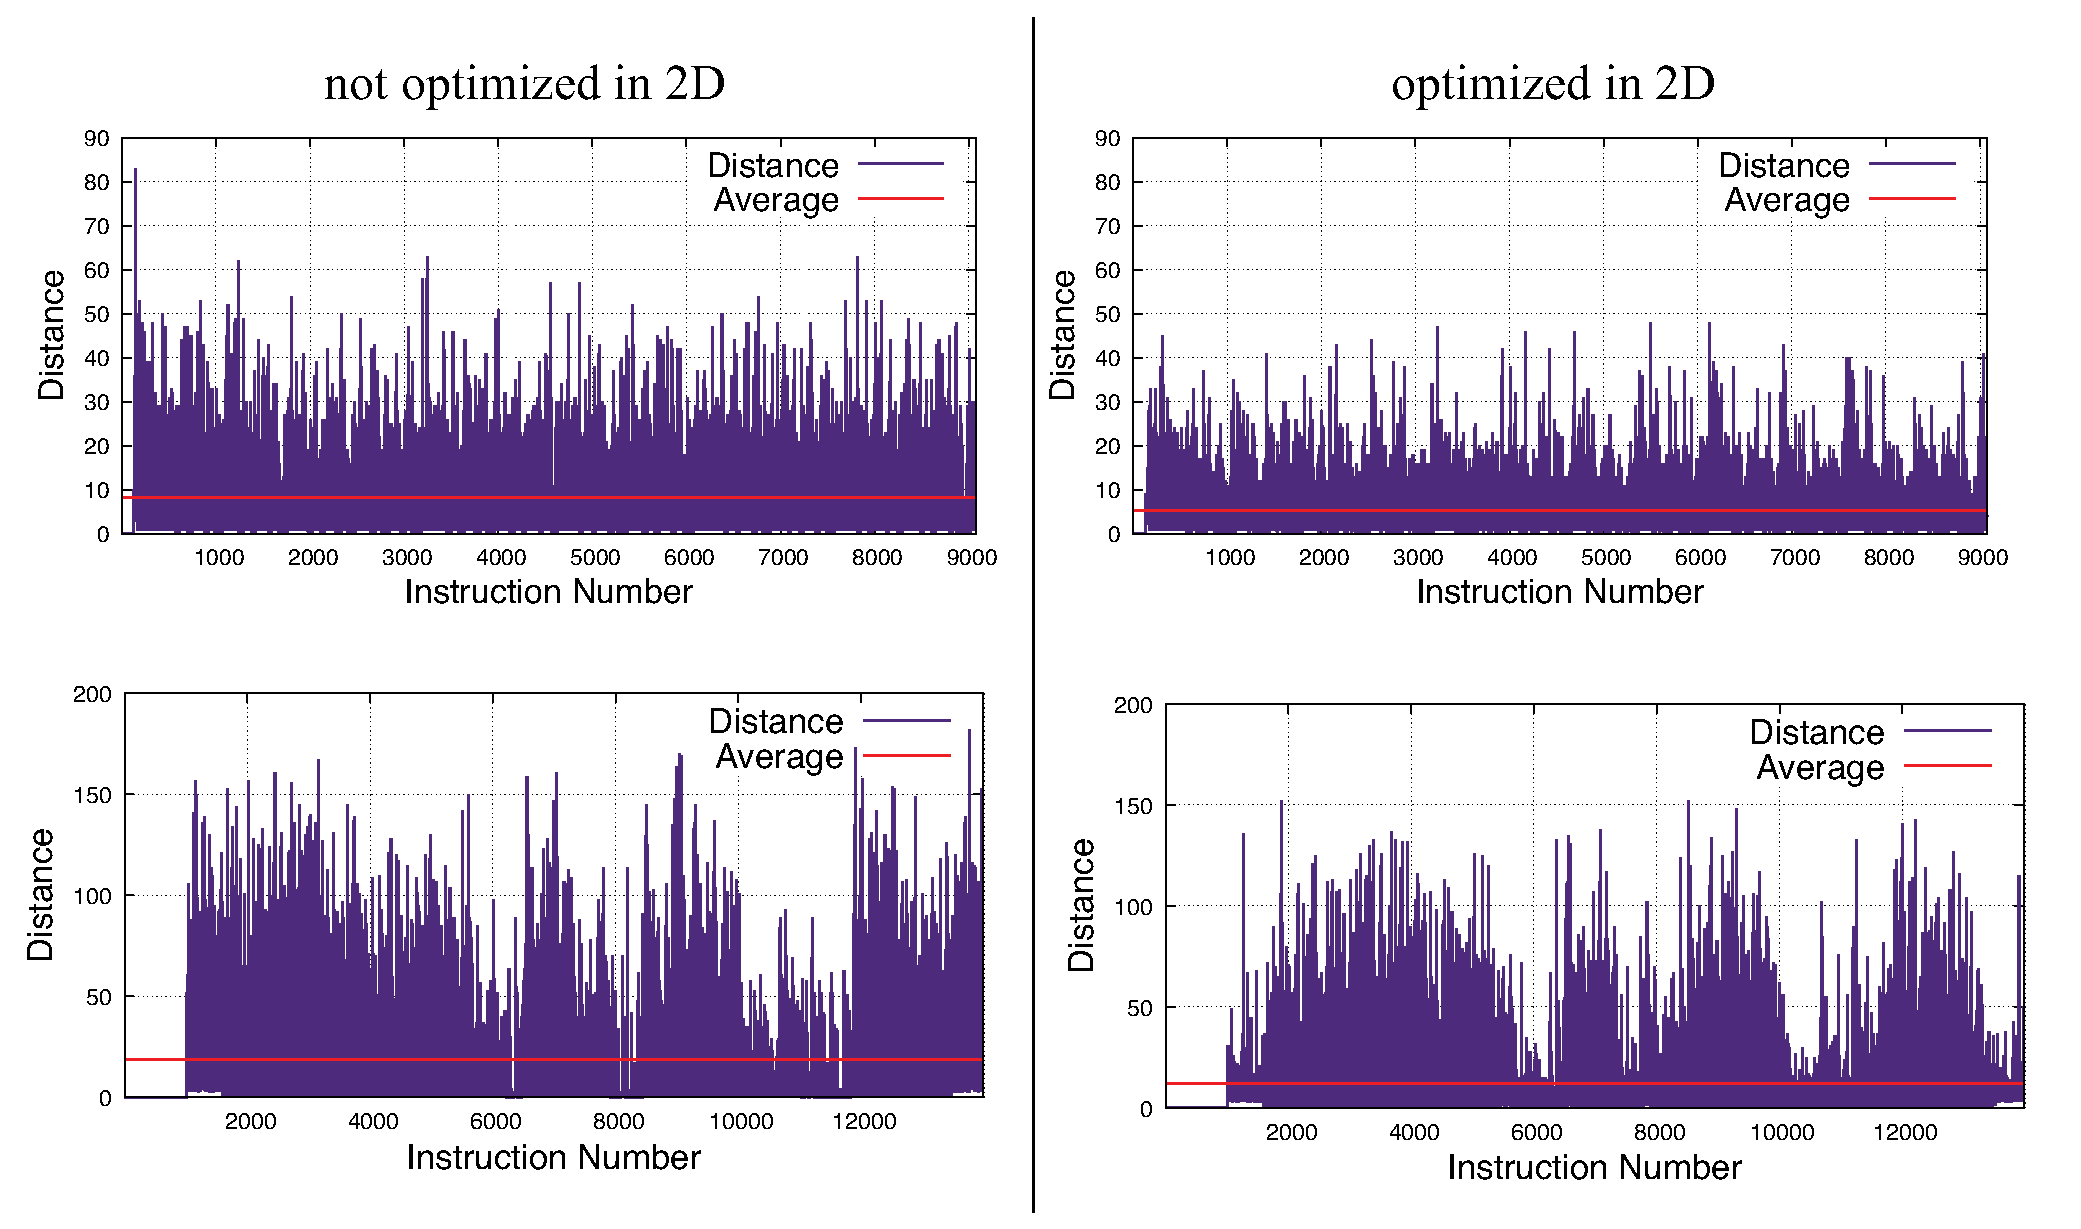
\includegraphics[scale=0.5]{figure/placement_optimization_2D.eps}
        \vspace{-20pt}\caption{}
        \label{placement_optimization_2D}
    \end{figure}
    
    \begin{figure}[h]
        \centering
        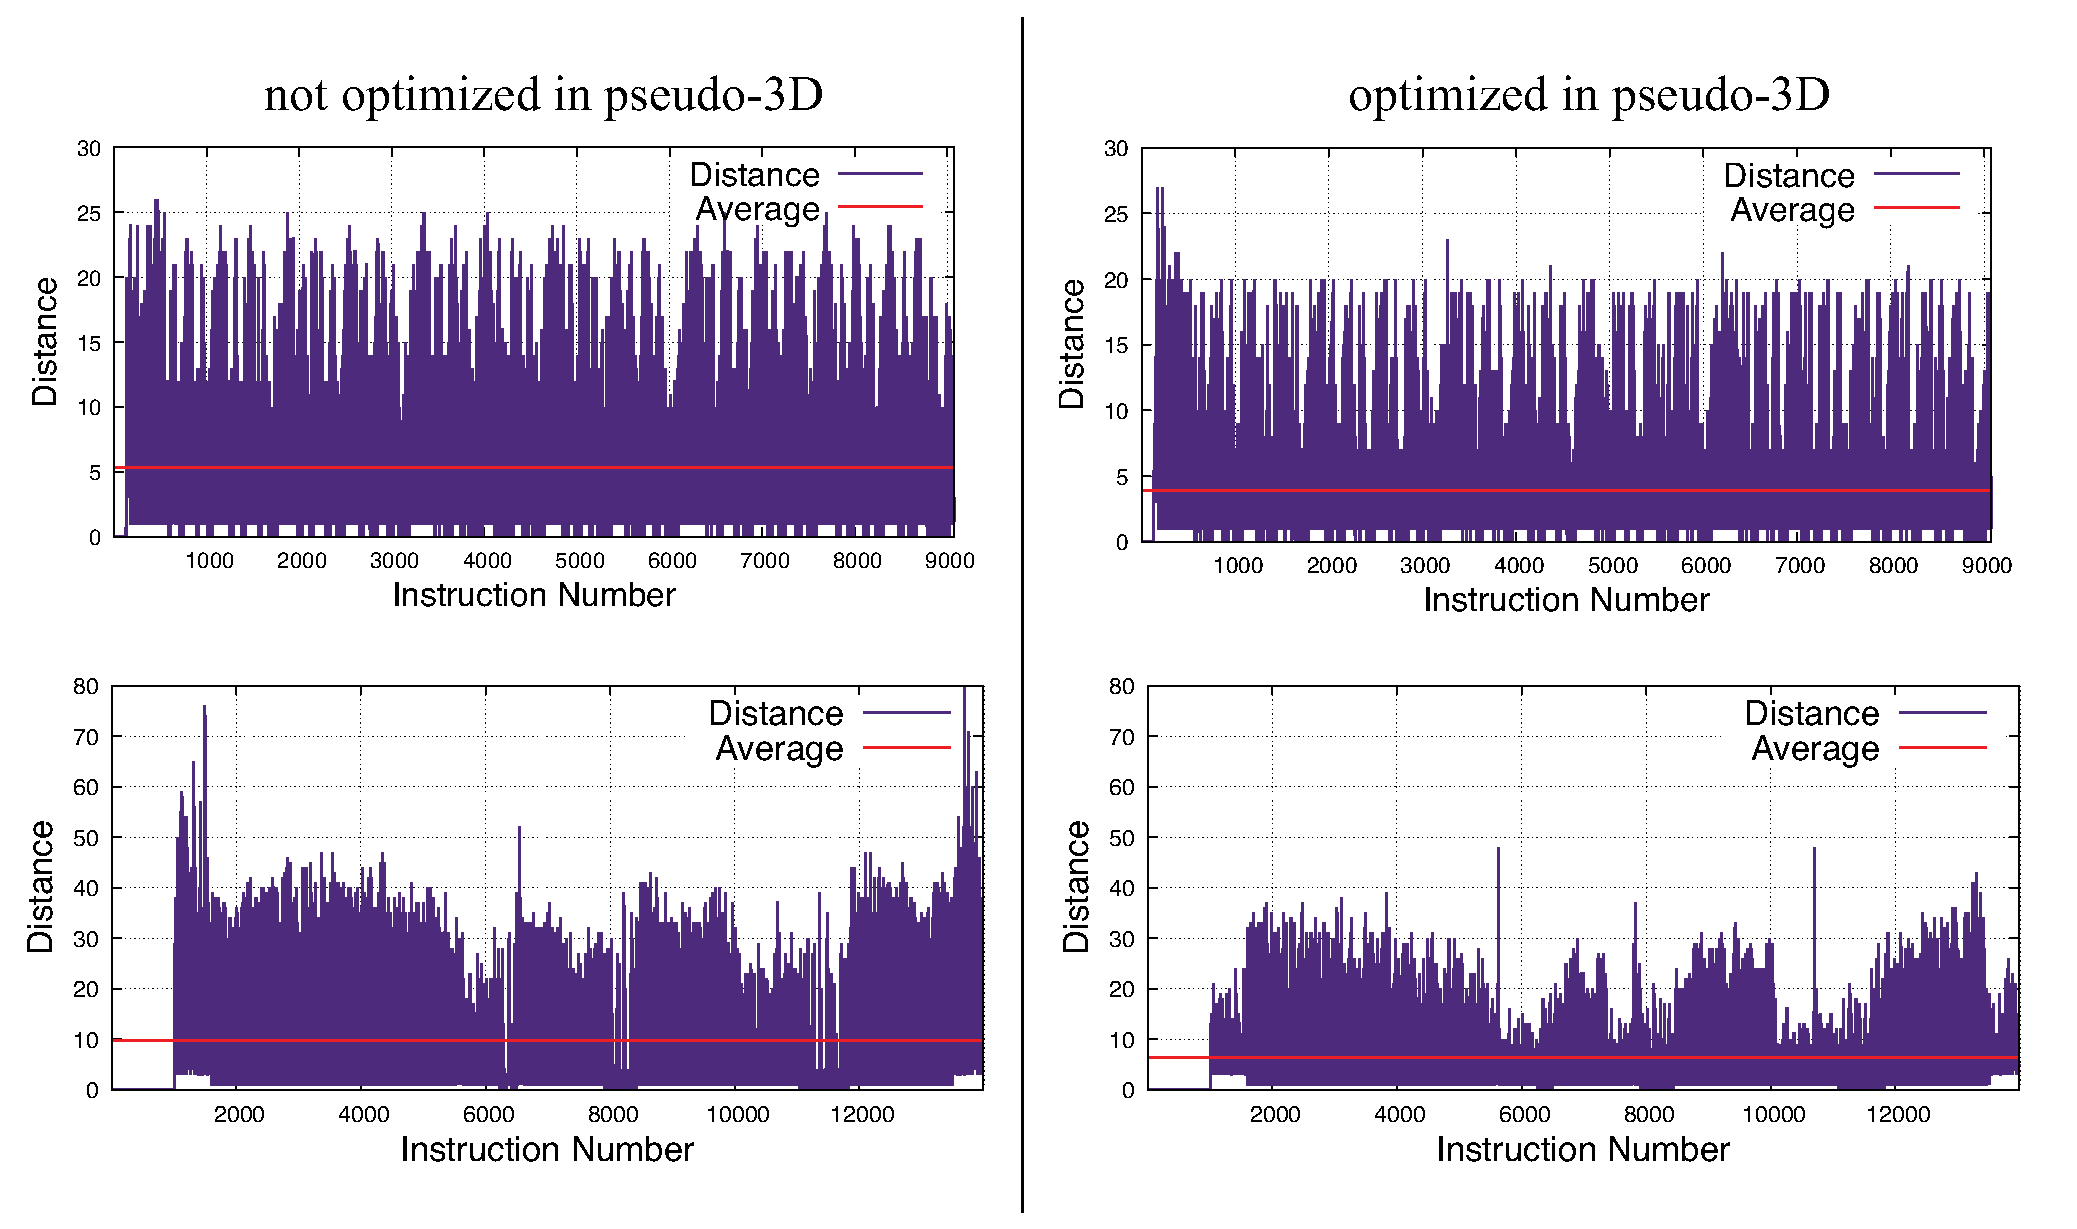
\includegraphics[scale=0.5]{figure/placement_optimization_3D.eps}
        \vspace{-20pt}\caption{}
        \label{placement_optimization_3D}
    \end{figure}
    \clearpage

    \begin{figure}[h]
        \centering
        \includegraphics[scale=0.60]{figure/graph_2D.eps}
        \vspace{0pt}\caption{}
        \label{graph_2D}
        \includegraphics[scale=0.60]{figure/graph_3D.eps}
        \vspace{0pt}\caption{}
        \label{graph_3D}
    \end{figure}
}

\end{document}